%% 
%% Copyright 2019-2020 Elsevier Ltd
%% 
%% This file is part of the 'CAS Bundle'.
%% --------------------------------------
%% 
%% Template article for cas-sc documentclass for 
%% single column output.

\documentclass[a4paper,fleqn]{cas-sc}
\pdfminorversion=7

\usepackage{tablefootnote}
\usepackage{appendix}
\usepackage{threeparttable}
\usepackage{afterpage}
\usepackage[table]{xcolor}
\usepackage{float}
\usepackage[authoryear]{natbib}
\usepackage{caption}
\captionsetup{format=plain, indention=0pt}
\captionsetup[figure]{font=small,labelfont=bf}
\hypersetup{
	colorlinks=true,
	linkcolor=blue,
	filecolor=magenta,      
	urlcolor=cyan,
	citecolor=blue,
}
\usepackage{tabularx}
\usepackage{tabulary}
\usepackage[above]{placeins}
\usepackage{microtype}
\setlength{\emergencystretch}{2em}
\usepackage{xr}
\externaldocument[supp-]{supplement}
% Non-floating table blocks inside a common figure/table result float.
% They use the CAS table caption, retain independent counters and labels,
% and allow the visual summary and its exact values to stay on the same page.
\ExplSyntaxOn
\NewDocumentEnvironment{resulttable}{}
  {\begin{minipage}{\linewidth}
   \__reset_tbl:
   \dim_set:Nn \l_tbl_width_dim {\linewidth}
   \cs_set:cpn {@captype} {table}
   \cs_set_eq:cN {@makecaption} \__make_tbl_caption:nn
   \centering\small}
  {\end{minipage}}
\ExplSyntaxOff

\usepackage[nameinlink]{cleveref}
\Crefname{figure}{Fig.}{Figs.}
\crefname{figure}{fig.}{figs.}
\Crefname{equation}{Eq.}{Eqs.}

%%%Author macros
\def\tsc#1{\csdef{#1}{\textsc{\lowercase{#1}}\xspace}}
\tsc{WGM}
\tsc{QE}
\tsc{EP}
\tsc{PMS}
\tsc{BEC}
\tsc{DE}
%%%

\begin{document}
\ExplSyntaxOn
\bool_gset_true:N \g_stm_nologo_bool
\ExplSyntaxOff
\let\printorcid\relax
\let\WriteBookmarks\relax
\def\floatpagepagefraction{1}
\def\textpagefraction{.001}
\setcounter{topnumber}{4}
\setcounter{bottomnumber}{4}
\setcounter{totalnumber}{10}
\renewcommand{\topfraction}{0.95}
\renewcommand{\bottomfraction}{0.95}
\renewcommand{\textfraction}{0.05}
\renewcommand{\floatpagefraction}{0.9}

\shorttitle{Auditing LLM-Derived Traveler Responses}
\shortauthors{A. Xu et al.}

\title [mode = title]{Beyond Static Imitation: Auditing LLM-Derived Traveler Responses for Transport Simulation}

\author[1]{An Xu}
\ead{AnX.RTL2324@tum-asia.edu.sg}

\author[2]{Zekai Jin}

\author[2]{Chengbo Zhang}


\author[1]{Yunfei Yin}
\cormark[1]
\ead{yunfeiyin@hit.edu.cn}

\address[1]{School of Transportation Science and Engineering, Harbin Institute of Technology, Harbin 150090, China}
\address[2]{Department of Civil Engineering, McGill University, Montreal, QC H3A 0C3, Canada}

\cortext[cor1]{Corresponding author: Yunfei Yin (yunfeiyin@hit.edu.cn).}

\begin{abstract}
Transport scenario analysis requires traveler models that reproduce changes in choices, not only baseline predictions. For models distilled from large language models (LLMs), agreement with a Teacher does not establish agreement with travelers or preservation of responses in simulation. We develop a response-centric evaluation that links three comparisons: paired Teacher--Student contrasts, agreement with stated choices, and transmission through assignment and network execution. A persona-disjoint benchmark from one LLM Teacher contains 398 test response pairs across six synthetic personas, evaluated with three neural training seeds. Explicit response supervision reduces mean absolute probability-response error from 0.06930 to 0.06586; a multinomial logit Student reduces it further to 0.05644. Pairing the logit model with independent neural timing yields a departure error of 7.61 minutes against the Teacher. The model ranking changes when evaluated on stated-choice convenience samples of 332 Singapore and 321 Shanghai respondents. For poorer public-transport accessibility in Singapore, the Teacher-best Student predicts a 13.85-percentage-point increase in PT use, whereas respondents report a 24.40-point decrease. A 1,000-traveler Helsinki execution experiment further separates response preservation from routability: feasibility-constrained assignment removes unroutable PT assignments without reducing the response gap under a perceived-delay perturbation. These results establish distinct tests for compression fidelity, agreement with stated behavior and execution consistency. Model selection for transport simulation should evaluate the relevant intervention response at each level rather than rely on a single imitation or prediction score.
\end{abstract}

\begin{keywords}
behavioral distillation \sep response fidelity \sep large language models \sep stated choice \sep agent-based transport simulation
\end{keywords}
\maketitle
\section{Introduction}
\label{sec:intro}
Suppose a transport planner wants to know how passengers would respond to a less reliable bus service. A model might reproduce today's public-transport share and still predict the wrong change tomorrow. It might also predict a reasonable change that disappears when travelers are assigned to routes and vehicles. Scenario analysis therefore needs more than an accurate baseline: it needs a defensible account of how choices change and how those changes reach the network \citep{horni2016multi}.

Large language models (LLMs) offer a flexible way to describe such choices. They can combine a traveler's circumstances with trip attributes and contextual information in a single prompt. Recent work uses this capacity for travel prediction, route choice and agent-based modeling \citep{mo2026llmtravel,wang2025agentic,liu2025framework}. Repeatedly querying an LLM for a simulated population is costly, however. Behavioral distillation addresses this problem by fitting a compact local model, the \emph{Student}, to judgments elicited from an LLM, the \emph{Teacher}. The Student can then generate travel choices without a live LLM call for every decision.

What should survive this compression? Conventional evaluation asks whether the Student matches the Teacher at individual input states. Transport scenario analysis also asks whether it preserves the change between two states: the same person making the same trip under different conditions. We call the first property \emph{static fidelity} and the second \emph{response fidelity}. Exact agreement at every state would imply exact agreement in every response. With limited data and model capacity, an average static score does not directly assess the particular changes a planner needs.

\begin{figure}[pos=htbp]
\centering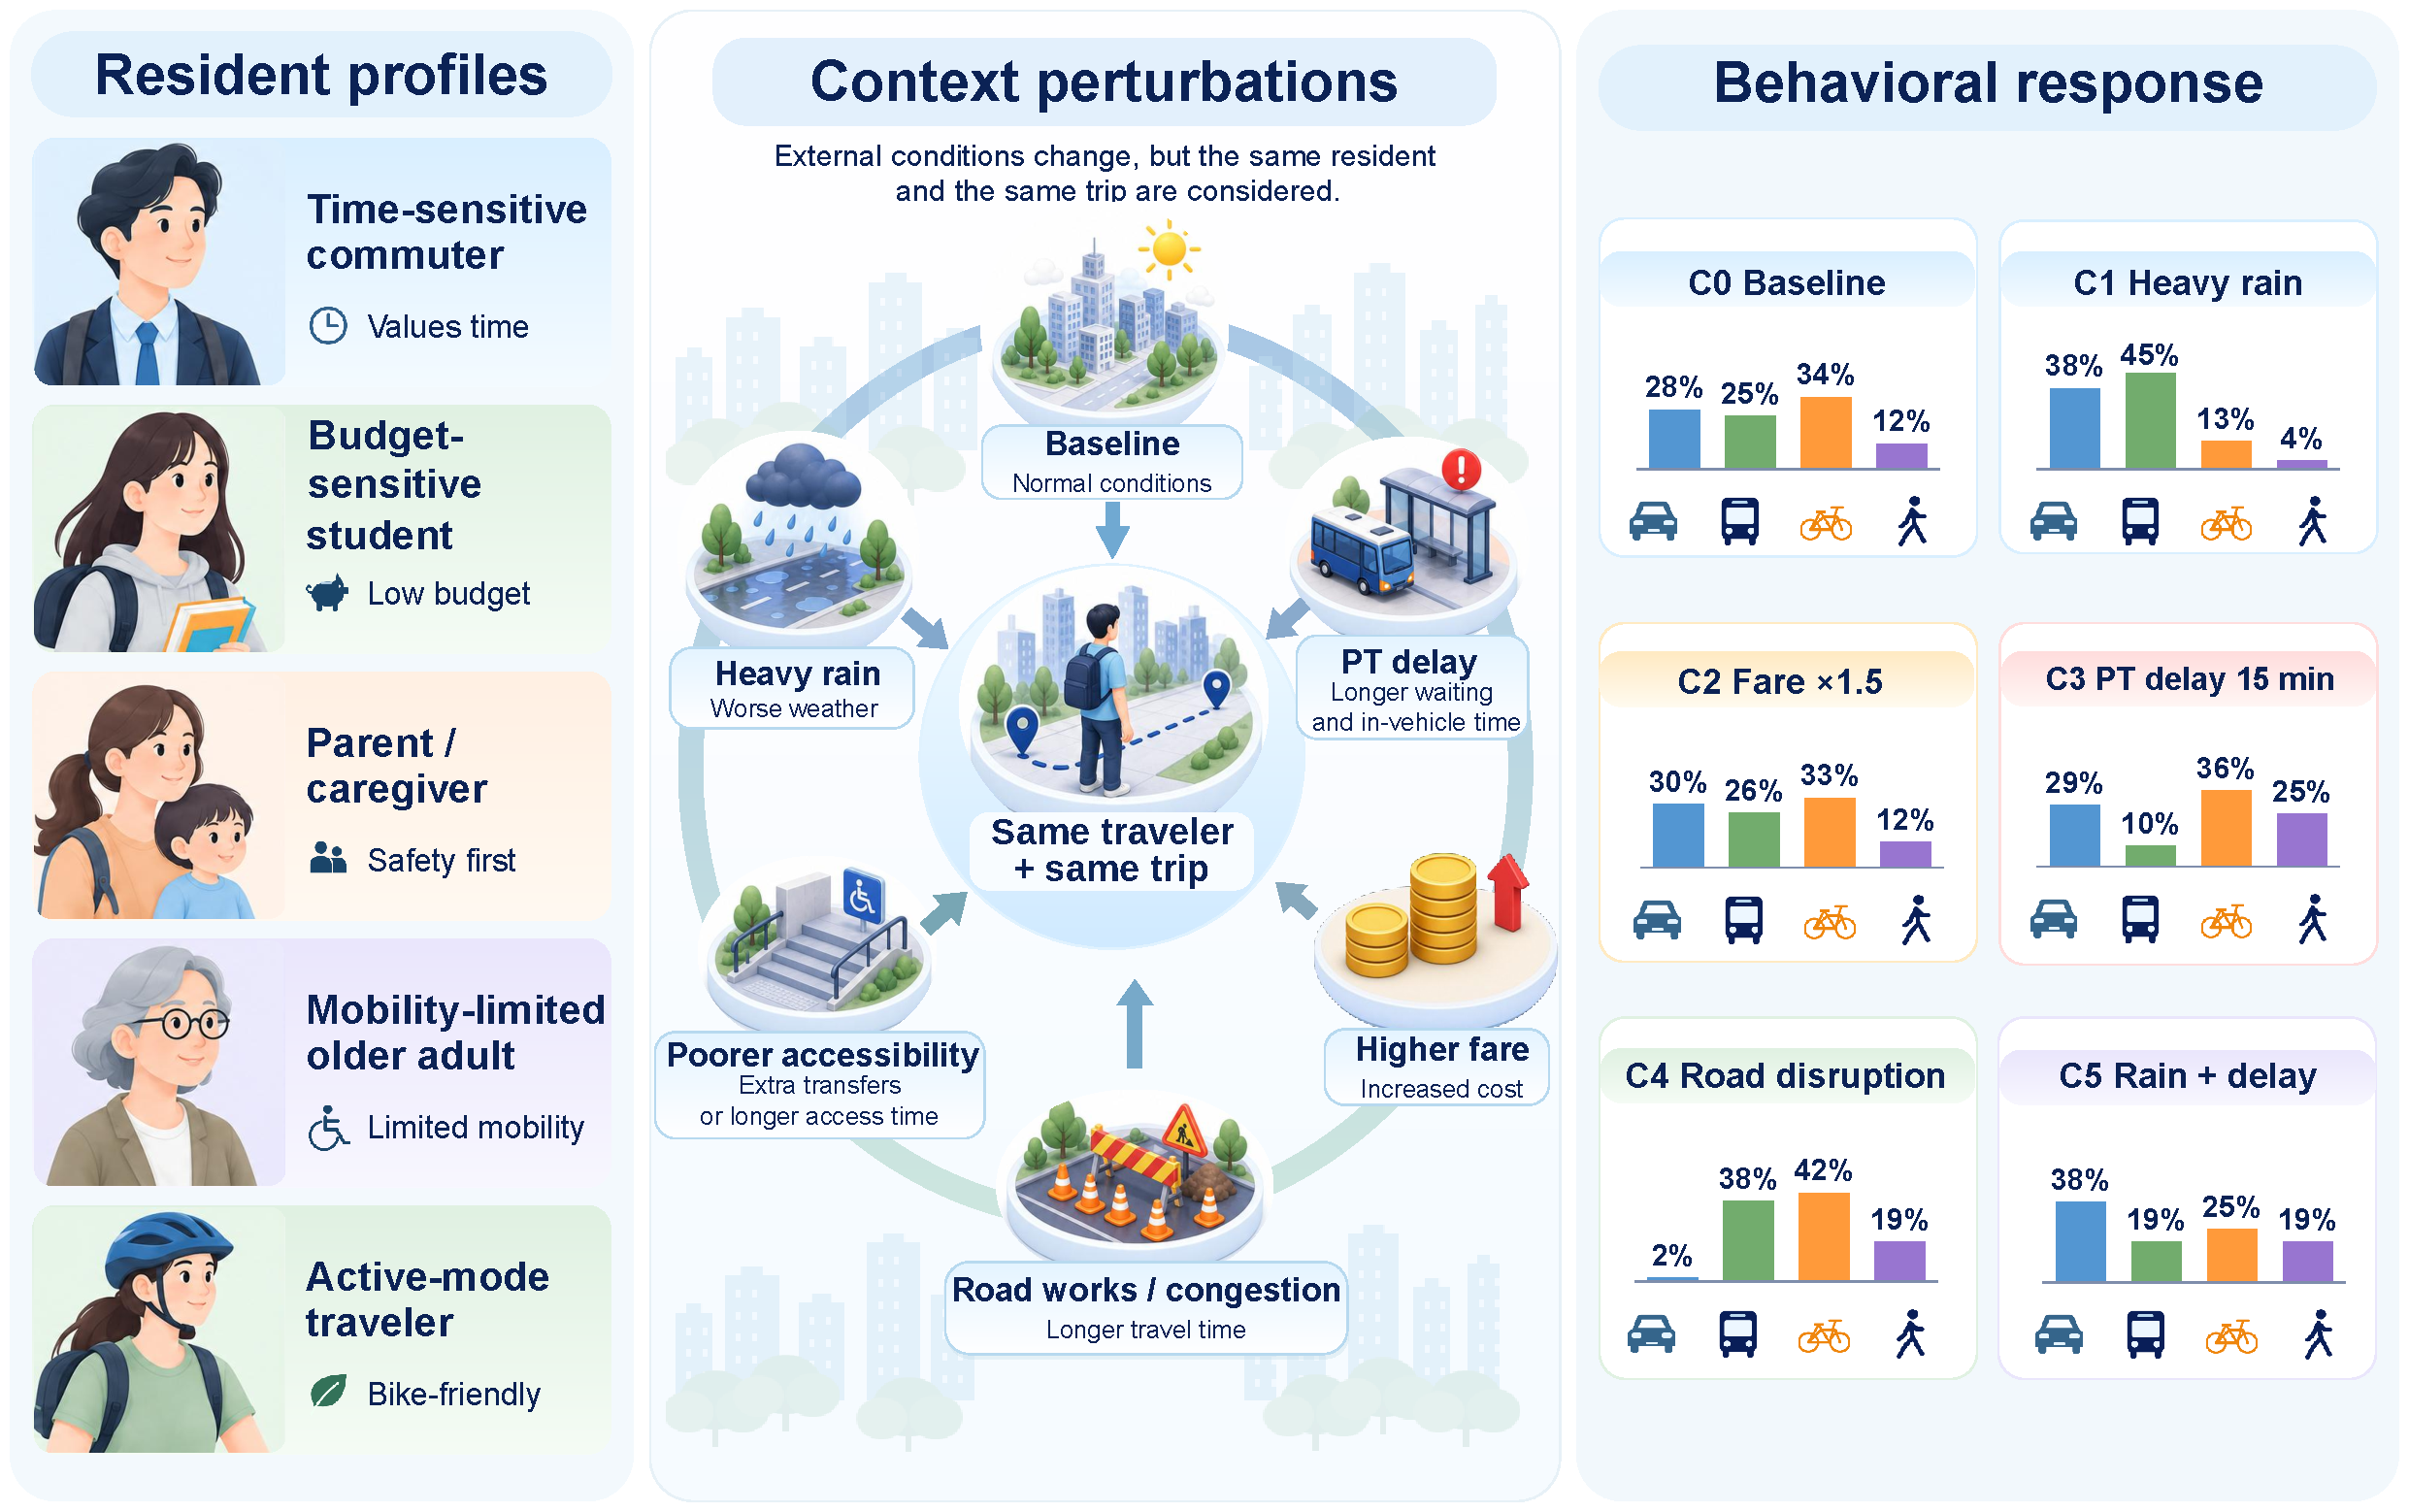
\includegraphics[width=0.95\textwidth,keepaspectratio]{figures/narrative/figure1_response_concept.pdf}
\caption{Traveler--trip pairing and illustrative demand responses. Each pair changes travel conditions while holding the traveler and trip fixed. Profiles are illustrative; bars are rounded, pre-routing mode assignments for 10,000 synthetic Singapore travelers, not survey observations. They use the supply-adapted model defined in Section~\ref{sec:architectures}. Poorer accessibility is evaluated separately. Scenario definitions and exact shares are in Supplementary Table~\ref{supp-tab:singapore}.}
\label{fig:concept}
\end{figure}

Preserving a Teacher's response is only the first test. An LLM can differ from people, and a faithful Student can retain that difference. Research on travel choice and synthetic respondents has already shown why predictive success and plausible language require separate behavioral checks \citep{wang2020deep,martinbaos2023prediction,bisbee2024synthetic,liu2026persona}. A further test arises in simulation: predicted probabilities must become assigned modes, feasible routes and actual boardings. Each step can alter the response. Figure~\ref{fig:concept} illustrates the paired traveler--trip comparison and its connection to aggregate demand.

We examine this chain using matched distillation experiments, stated-choice surveys in Singapore and Shanghai, and controlled network execution in Helsinki. Response supervision is tested against the same archived endpoint targets used by ordinary distillation. A new synthetic-persona experiment examines agreement with a later API model, including a setting where delay-related training examples are withheld. The surveys test the resulting models against people's stated responses. Finally, a four-arm simulation distinguishes a perceived delay from a physical reduction in transit service. These settings provide complementary evidence; they are not a cross-city prediction benchmark.

The findings reveal where a favorable comparison stops carrying over. Response supervision helps within covered tasks, but its advantage reverses on withheld delay scenarios. The Student closest to the archived Teacher can predict the opposite direction to a stated human response. In the network, perceived delay and fewer scheduled trips produce markedly different demand changes. Our contribution is an empirical evaluation of these boundaries and a practical way to locate them. The learning objectives and modular models serve as controlled comparisons within that evaluation, rather than as a claim that a new loss solves behavioral validity.

\section{Related work}
\label{sec:related}
\subsection{LLM traveler models and empirical alignment}
LLMs have been used to generate activities and travel in urban simulation \citep{gatsim2026,genagents2026}, model day-to-day route choice \citep{wang2025agentic}, and predict modes using retrieved examples or incremental learning \citep{ragbenchmark2026,incremental2026}. Conceptual work has set out their possible roles within transport systems and motivated hybrid designs \citep{liu2025framework,nie2025roles}. These applications establish the relevance of LLM-generated decisions; they do not make fidelity to an LLM equivalent to fidelity to travelers.

Empirical alignment is a separate research problem. Studies of synthetic survey respondents document both reproducible aggregate patterns and sensitivity to prompts and model versions \citep{argyle2023out,aher2023using,bisbee2024synthetic}. For travel choice, \citet{valuingtime2026} examine the direction and magnitude of time trade-offs, while \citet{liu2026persona} learn persona-based representations using empirical choices. In this journal, \citet{xu2026satisfaction} compare zero-shot and few-shot LLM predictions of travel satisfaction and study improvements from task-specific examples. Learning and adjustment behavior have also been addressed explicitly \citep{dualagent2026}. These studies motivate empirical checks rather than treating the Teacher as a behavioral ground truth.

The distinction in the present study is the object being audited: a numerical Student fitted to archived LLM judgments. We evaluate whether its finite responses match those judgments and whether this ranking transfers to independently collected stated responses. The human comparison is an external evaluation, not a calibration procedure. The contemporary LLM subset is a later reference model and does not, without matched backend provenance, identify how much discrepancy originated during compression.

\subsection{Predictive and behavioral criteria for choice models}
Random-utility models connect choice probabilities to traveler characteristics and alternative attributes \citep{mcfadden1974conditional,ben1985discrete}. Generalized and mixed logit formulations represent richer heterogeneity \citep{walker2002generalized,hensher2003mixed,train2009discrete}, while representation learning can retain a specified utility core alongside flexible components \citep{sifringer2020enhancing}. Comparisons of these families show that predictive performance, market shares and behavioral indicators can favor different models \citep{wang2020deep,martinbaos2023prediction}.

Distillation changes the estimation target from observed choices to another model's elicited distributions. A structured utility model may preserve such responses through regularization and restricted functional form, without demonstrating that the Teacher or travelers follow that form. We therefore compare logit and neural specifications on the same information, then evaluate their human-response discrepancies separately. Independent timing predictors test whether choice and departure adjustment benefit from different specifications rather than assuming that a shared representation is preferable for both.

\subsection{Response supervision and simulation surrogates}
Knowledge distillation transfers predictions or representations to a smaller model \citep{hinton2015distilling,gou2021knowledge,sanh2019distilbert}. Relational distillation preserves relationships between examples \citep{park2019relational}; Sobolev training uses output and derivative information \citep{czarnecki2017sobolev}. Response-aware fitting is therefore not a new general principle. Here the relation is a finite, travel-specific difference between elicited distributions. It is calculated from endpoint targets already available to every controlled Student, so the experiment concerns an optimization preference for scenario contrasts rather than access to additional Teacher information.

Surrogate modeling also has an established transport role. \citet{natterer2025surrogates} approximate network outcomes of a MATSim model to accelerate scenario exploration. Our Student instead replaces the traveler decision function while retaining network construction and execution. This distinction makes assignment and routing part of the evaluation rather than outputs that the surrogate directly predicts. A concurrent preprint, CALM, combines calibrated choice, optional LLM planning, network feedback and replayable evaluation \citep{cheng2026calm}. Its system-level integration is complementary to our narrower question: whether finite responses survive compression and whether the resulting model ordering persists across Teacher, stated-choice and execution comparisons. Neither the use of an LLM in a simulator nor the presence of intervention tests alone constitutes the contribution claimed here.

\section{Evaluating and learning traveler responses}
\label{sec:method}
\subsection{The response as the object of comparison}
\label{sec:states}
A traveler state $\mathbf x$ describes a person, a trip, contextual conditions and attributes of four alternatives: private car, public transport (PT), bicycle and walking. Attributes include time, cost, weather exposure and the components of a PT journey. A model returns a normalized choice distribution $\mathbf p(\mathbf x)$ and a departure-time adjustment. The distribution is a model output, not an established human choice frequency. Appendix~\ref{sec:supp_inputs} explains the inputs and the survey encodings.

For two states that hold the person and trip fixed, the response is
\begin{equation}
\Delta\mathbf p_j=\mathbf p_j(\mathbf x')-\mathbf p_j(\mathbf x),\qquad j\in\{T,S\}.
\label{eq:response}
\end{equation}
Here $T$ and $S$ denote Teacher and Student. We evaluate the absolute difference between their responses, averaged over modes available in either state and then over paired states:
\begin{equation}
E_{\Delta p}=\frac{1}{N}\sum_{i=1}^{N}\frac{1}{|\mathcal A_i|}
\sum_{m\in\mathcal A_i}|\Delta p_{S,im}-\Delta p_{T,im}|.
\label{eq:response_metric_main}
\end{equation}
Lower error means closer agreement in the specified change. This finite contrast does not by itself estimate a population causal effect or an elasticity. Static KL divergence measures endpoint agreement, departure MAE measures timing agreement, and an interaction contrast asks whether two perturbations combine in the same way. Supplementary Section~\ref{supp-sec:metric_definitions} gives the additional definitions.

\subsection{Controlled and adapted Students}
\label{sec:architectures}
The joint neural Student encodes the traveler and the attributes of each alternative, scores the alternatives and normalizes over the available modes. It shares these representations with a departure predictor. The multinomial logit Student (MNL-S) instead uses linear choice utilities on the same structured information. Separate ridge, bounded-linear and neural timing predictors allow choice and departure adjustment to favor different specifications. The neural outputs are bounded to an hour in either direction. Appendix~\ref{sec:model_details} explains the model roles; detailed dimensions and fitting settings are in Supplementary Section~\ref{supp-sec:supp_controlled}.

We also evaluate a frozen supply-adapted Student (SA-Student). This model was adapted with additional PT attributes and contrasts between contexts, travelers and accessibility levels. Its training history and availability treatment differ from those of the controlled Students. It therefore provides a deployment case, not an isolated test of the response penalty (Appendix~\ref{sec:s9_recipe}).

\subsection{Response-aware fitting}
\label{sec:loss}
The soft-KL baseline fits the Teacher distribution and departure adjustment at both endpoints of every training pair. Signed-response fitting adds a weighted penalty on the difference between the Teacher and Student changes:
\begin{equation}
\mathcal L=\mathcal L_{\mathrm{endpoint}}+\lambda\mathcal L_{\mathrm{response}}.
\label{eq:training_objective}
\end{equation}
The response penalty is a batch average over available mode--pair entries. We compare direct signed absolute error with a penalty that separates direction and magnitude. An additional CE+KL comparator fits the Teacher's most likely mode as a hard label. All controlled neural objectives receive the same endpoint information. Thus paired supervision changes what the optimizer prioritizes; it does not supply new Teacher knowledge. Appendix~\ref{sec:loss_diagnostics} gives the exact losses and their limitations, including a flat region in the direction-plus-magnitude penalty.

\subsection{Human responses and network execution}
\label{sec:execution_method}
For a survey contrast, the human response is the change in the share selecting the relevant mode or mode group. The corresponding model response is the change in its predicted probability, averaged over the same respondents. We report their difference as \emph{response bias}: positive values mean a more positive model response, and negative values a more negative one. Full task sets are retained together when resampling respondents.

An API reference queried on the same survey tasks provides a further descriptive comparison. On the same people and contrasts,
\begin{equation}
S-H=(T_{\mathrm{now}}-H)+(S-T_{\mathrm{now}}),
\label{eq:attribution}
\end{equation}
where each term is a mean response. This identity separates two observed discrepancies. Because $T_{\mathrm{now}}$ was queried later, it does not identify the historical error introduced by compression.

In simulation, we trace PT use from predicted probabilities through feasibility adjustment, mode assignment, routing and boarding. A feasible route is one returned by the specified direct-or-one-transfer search, rather than proof that all other connections are impossible. Deterministic assignment takes the most probable mode; stochastic assignment samples the probabilities; feasibility-constrained sampling first removes unavailable or unroutable alternatives and renormalizes. Without that correction, a failed car, bicycle or PT route triggers a walking fallback. Predictions remain fixed during each simulation run.

Every stage uses the initial population as denominator. If $R$ denotes a change from baseline, the predicted-to-simulated gap is
\begin{equation}
G=R^{\mathrm{sim}}-R^{\mathrm{pred}}
=(R^{\mathrm{adj}}-R^{\mathrm{pred}})+(R^{\mathrm{sim}}-R^{\mathrm{adj}}).
\label{eq:execution_decomposition}
\end{equation}
This separates a change to the sampling distribution from subsequent execution. Boarding and journey completion remain distinct outcomes. The departure adjustment is applied before route feasibility is checked, so timing can change the itinerary even if it leaves the binary feasibility indicator unchanged. Appendix~\ref{sec:execution_support} explains the execution controls and the geometry of the feasibility correction.

\section{Evidence and experimental design}
\label{sec:design}
Table~\ref{tab:study_design} distinguishes the data used to learn a model from the evidence used to evaluate it. Neither human survey is used for training or selection. Training seeds, repeated API responses and repeated assignments describe different sources of variability and are never counted as additional people.
\begin{table}[pos=htbp]
\caption{Evidence sources and the unit behind each comparison.}\label{tab:study_design}
\small\renewcommand{\arraystretch}{1.15}
\begin{tabularx}{\linewidth}{@{}p{.23\linewidth}p{.28\linewidth}X@{}}\toprule
Question & Independent units & What is compared \\\midrule
Compression fidelity & Six held-out personas; 398 pairs & Matched objectives and specifications against archived Pro targets \\
Response outside training coverage & Thirty new personas; pilot kept separate & Full and delay-withheld Students against a later Go Flash reference \\
Agreement with people & 332 Singapore and 321 Shanghai respondents & Within-person stated responses; later Pro reference on 24 people per city \\
Transmission through supply & 1,000 fixed synthetic travelers & Assignment rules and four supply arms; paired assignment seeds \\\bottomrule
\end{tabularx}
\end{table}


\subsection{Archived targets and matched training}
\label{sec:controlled_design}
The archived benchmark contains disjoint training, validation and test groups of synthetic traveler profiles, here called personas. The test set has 398 response pairs from six personas. Within each training seed, controlled neural models share initialization, architecture, endpoint targets, pair order and optimization budget. The primary choice-model selector minimizes validation macro-source KL, giving each supervision source a role in selection. A response-based selector and a grid of response-loss weights test sensitivity. MNL-S regularization is selected on the same validation criteria. Departure predictors are selected separately by departure MAE, so timing comparisons do not silently change the choice-selection rule. Appendix~\ref{sec:optimization_support} and Supplementary Section~\ref{supp-sec:supp_controlled} document these comparisons.

The original split also withholds a fare--congestion combination while retaining its constituent factors. We audited endpoints, references and linked contrast units to confirm that the held-out combination does not enter training or validation. This is a compositional test. To test a stronger omission, we additionally remove positive-delay endpoints and entire delay-mechanism groups from training and validation, refit feature statistics, and retrain soft-KL and signed-response models. Budgets are matched between methods within each setting. The full and delay-withheld settings have different retained data and update counts, so their difference does not isolate removal of the intervention family as a pure causal factor.

Archived Teacher targets were collected through the official DeepSeek V4 Pro service, according to the authors' collection records and confirmation. The later same-task survey campaign also requested and returned \texttt{deepseek-v4-pro}. Repeated valid vectors are averaged within state. We preserve these targets as the reference for compression; service names alone do not certify an immutable backend across collection periods.

\subsection{A new synthetic-persona reference test}
\label{sec:new_reference_design}
A separate experiment evaluates the frozen Students on new persona profiles, one fixed numerical trip and a common set of travel conditions. Twelve pilot personas are used only for sample-size planning; thirty different personas form the formal sample. Each has a baseline and eleven changes covering delay, fare, access, combinations, rain and PT infeasibility. Three valid API responses are averaged per state. Profiles are excluded from all prior persona sets. The fixed trip and inherited feasible supply profile limit interpretation to these inputs, rather than geographic or population generalization.

This new reference was supplied by OpenCode Go with requested and returned model \texttt{deepseek-v4.1-flash}. It therefore measures agreement with a different API model, not compression error against the original Pro Teacher. The primary contrast, defined before formal collection, is signed-response minus soft-KL error under full training and KL selection. We average the paired differences over contrasts and training seeds within persona, then bootstrap personas. Delay-family and individual-condition comparisons are descriptive, with pointwise intervals. The pilot is excluded from formal estimation. Appendix~\ref{sec:new_protocol} gives the precision rule, acquisition settings and a post-hoc service-metadata diagnostic. No samples were excluded because of that diagnostic.

\subsection{Independent stated-choice evaluation}
\label{sec:human_design}
The Singapore analysis includes 332 residents and the Shanghai model comparison includes 321 respondents. Each completed ten stated-choice tasks. Recruitment through personal contacts and onward sharing produced convenience and snowball samples; the target is agreement within these samples, not citywide demand. Singapore data were collected from 20 August to 5 September 2026 and Shanghai data from 12 to 18 September 2026. Appendix~\ref{sec:supp_inputs} gives eligibility, sample flow and the tasks.

Singapore respondents saw numerical time-and-cost tables. Most Shanghai conditions were qualitative, so unreported durations require numerical reference values for model evaluation. Those assumptions were defined without reference to the human answers. We examine alternative input specifications and a separate network-derived-input diagnostic. All explicit choices are scored, including choices unavailable under the model's ownership rule. The two Shanghai answers indicating no suitable mode are excluded from four-mode scoring. Human-only sensitivity retains eligible respondents outside the model's input mapping.

Within-person contrasts compare stated mode changes with probability changes. Respondent bootstraps retain each person's complete task set and use shared resamples across models. We report nominal 95\% intervals and family-adjusted intervals over the contrasts in each city. Seed variability is separate. An additional same-input API comparison uses 24 respondents per city, with three valid queries per task and no access to their answers. This later Pro reference supports Eq.~\ref{eq:attribution}; it is distinct from both archived supervision and the new Go synthetic sample.

\paragraph{Ethics and consent statement.} The stated-choice questionnaires were administered as anonymous, minimal-risk surveys. No direct personal identifiers were collected. Before beginning the questionnaire, all participants were shown an electronic information and consent statement describing the study purpose, voluntary participation, intended research use of the responses, and confidentiality protections; only respondents who provided consent proceeded to the survey. Formal institutional ethics approval was not obtained. The study procedures were designed to protect participant privacy and to limit data collection to information necessary for the stated research purpose.

\subsection{Perceived conditions and physical transit supply}
\label{sec:execution_design}
The Helsinki experiments hold a synthetic population of 1,000 travelers fixed and use OSM roads and HSL timetables. The original experiment compares assignment rules under an added perceived PT delay while leaving physical supply unchanged. A four-arm extension distinguishes this input manipulation from an actual service reduction: baseline; perceived delay with the original timetable; reduced service with baseline behavioral predictions frozen; and reduced service with predictions recomputed from its level of service. The reduction removes alternating departures within line-and-stop-sequence groups, updating both the route-search index and the MATSim timetable. Delay is not added again to the reduced-service arms.

The extension uses feasibility-constrained assignment, SA-Student and MNL-S with a fixed independent neural timing predictor, and five paired assignment seeds. Its 40 configurations include verified reuse of 12 historical runs and 28 new runs. Responses are paired within person and seed; assignment seeds are averaged within person before person-level bootstrap resampling. This is a single-iteration execution experiment, with no feedback from experienced conditions to a subsequent behavioral decision. Network-derived active-mode speeds are retained, so journey times are diagnostic outputs, not calibrated predictions of the benefits of a service change. Appendix~\ref{sec:execution_support} and Supplementary Section~\ref{supp-sec:supp_execution} provide the stage definitions and additional controls.

\section{Results}
\label{sec:results}
\subsection{Response fidelity and behavioral specification}
\begin{figure}[pos=p]
\begin{resulttable}
\centering\small
\caption{Probability-response fidelity on the held-out Teacher benchmark.}
\label{tab:response_main}
\setlength{\tabcolsep}{4pt}
\renewcommand{\arraystretch}{1.12}
\begin{tabular*}{\linewidth}{@{\extracolsep{\fill}}lrrr@{}}
\toprule
Model / objective & Macro-source KL $\downarrow$ & Response error $\downarrow$ & Interaction error $\downarrow$ \\
\midrule
Soft KL & $0.0915\pm0.0187$ & $0.0693\pm0.0032$ & $0.0457\pm0.0038$ \\
CE+KL & $0.1046\pm0.0170$ & $0.0753\pm0.0016$ & $0.0518\pm0.0038$ \\
Signed response & $0.0871\pm0.0138$ & $0.0665\pm0.0050$ & $0.0465\pm0.0036$ \\
Direction+magnitude & $0.0861\pm0.0145$ & $0.0659\pm0.0042$ & $0.0464\pm0.0039$ \\
\midrule
MNL-S & $0.0731$ & $0.0564$ & $0.0386$ \\
\bottomrule
\end{tabular*}
\par\smallskip\begin{minipage}{\linewidth}\footnotesize
Neural entries are means $\pm$ SD over three training seeds. The test set contains 437 states, 398 response pairs and 94 interaction contrasts from six held-out synthetic personas. All models, including the MNL-S regularization, are selected by validation macro-source KL. MNL-S uses the same inputs and training states as the neural Students.
\end{minipage}
\end{resulttable}

\par\vspace{4pt}
\centering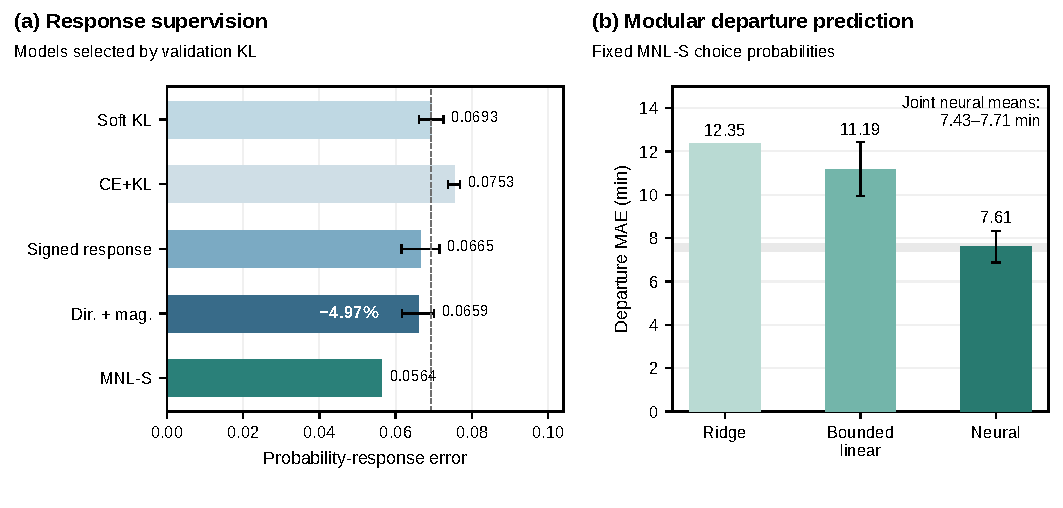
\includegraphics[width=\textwidth]{figures/narrative/figure3_response_timing.pdf}
\caption{Response learning and modular departure prediction. (a) Probability-response errors for models selected by validation KL. The dashed line marks soft KL. (b) Departure MAE of three timing predictors combined with the same MNL-S choice model, whose probabilities are identical across the three. The shaded band spans the means of the four joint neural models selected for timing (7.43--7.71~min). Error bars show training-seed SD where applicable. Departure targets are the Teacher's.}
\label{fig:response_learning}
\par\vspace{4pt}
\begin{resulttable}
\centering\small
\caption{Departure prediction under a common selection criterion (validation MAE).}
\label{tab:timing_main}
\setlength{\tabcolsep}{4pt}
\renewcommand{\arraystretch}{1.12}
\begin{tabular*}{\linewidth}{@{\extracolsep{\fill}}llrr@{}}
\toprule
Choice model & Departure predictor & Total parameters & MAE (min) $\downarrow$ \\
\midrule
Joint / soft KL & Shared neural encoders & 24,562 & $7.61\pm0.75$ \\
Joint / CE+KL & Shared neural encoders & 24,562 & $7.43\pm0.91$ \\
Joint / signed response & Shared neural encoders & 24,562 & $7.71\pm0.66$ \\
Joint / direction+magnitude & Shared neural encoders & 24,562 & $7.55\pm0.80$ \\
\midrule
MNL-S & Ridge regression & 555 & $12.35$ \\
MNL-S & Bounded linear & 555 & $11.19\pm1.24$ \\
MNL-S & Independent neural & 18,733 & $7.61\pm0.72$ \\
\bottomrule
\end{tabular*}
\par\smallskip\begin{minipage}{\linewidth}\footnotesize
Errors are measured against Teacher departure targets on the 437 test states. Neural and bounded-linear predictors report means $\pm$ SD over three training seeds, and the ridge fit is deterministic. MNL-S choice probabilities are identical across the three timing predictors. The joint models in this table are trained separately and selected by validation departure MAE, whereas those in Table~\ref{tab:response_main} are selected by validation KL.
\end{minipage}
\end{resulttable}

\end{figure}
Explicit response supervision improves finite-contrast fidelity under the matched benchmark protocol. Direction+magnitude lowers mean response error from 0.06930 under soft KL to 0.06586, a reduction of 4.97\% (Table~\ref{tab:response_main}; Figure~\ref{fig:response_learning}a). The paired difference is $-0.00345$, with a persona-clustered 95\% interval of $[-0.00504,-0.00191]$. Signed response reaches 0.06653. The difference between the two paired objectives is small ($-0.00067$, interval $[-0.00199,0.00072]$), which supports explicit response supervision but does not establish an additional benefit from separating sign and size.

The gain is distributed across the tested seeds and personas. Across the three training seeds, direction+magnitude differs from soft KL by $-0.00499$, $-0.00441$ and $-0.00094$, although the interval for the third seed includes zero. Averaged over seeds, the error is lower for each of the six test personas, and removing any one persona from evaluation leaves differences between $-0.00408$ and $-0.00310$ (Supplementary Tables~\ref{supp-tab:response_breakdown} and~\ref{supp-tab:response_seed_differences}). The advantage of both paired objectives also persists when the targets are recomputed from the available repeated Teacher outputs, an analysis that excludes the mechanism states for which repeats were not recovered.

The benefit is specific to single contrasts. For combined perturbations, the paired objectives reach interaction errors of 0.0465 and 0.0464, slightly above the 0.0457 of soft KL, so supervising individual responses did not improve interaction error in this benchmark. CE+KL has the largest response error, 0.07528, even though it fits an additional target. Its hard label pulls predictions toward the Teacher's leading mode, and in the fitted networks this enlarges the probability changes on pairs whose leading mode does not change (Supplementary Section~\ref{supp-sec:loss_diagnostics}). Fitting the most likely mode appears to distort the graded responses on which scenario analysis depends.

A change of specification matters more than any change of objective. MNL-S, fitted to the same endpoints with linear utilities, attains the lowest errors on all three measures: 0.05644 for response error, 0.07310 for macro-source KL and 0.03865 for interaction error. Its response error is 14.30\% below that of direction+magnitude, with a paired interval of $[-0.01246,-0.00722]$. One plausible reading is that structured utilities restrict how a change in an attribute can propagate to probabilities. With only 28 training personas, this restriction appears to generalize better than the additional freedom of the neural Students, which can fit individual states without reproducing the contrasts between them.

The linear specification is less suited to timing. With the MNL-S choice probabilities held fixed, ridge regression, the bounded linear predictor and the independent neural predictor give departure MAEs of 12.35, 11.19 and 7.61 minutes (Table~\ref{tab:timing_main}; Figure~\ref{fig:response_learning}b). The neural predictor brings the modular model within the 7.43--7.71-minute range of the joint models selected for timing, with 18,733 rather than 24,562 parameters. Choice and timing therefore favor different functional forms, and estimating them separately retains the response advantage of linear utilities with comparable departure errors in this benchmark. All timing errors are measured against Teacher targets, not observed departure behavior.

\FloatBarrier
\subsection{Agreement with stated responses}
\label{sec:human_results}
\begin{figure}[pos=p]
\centering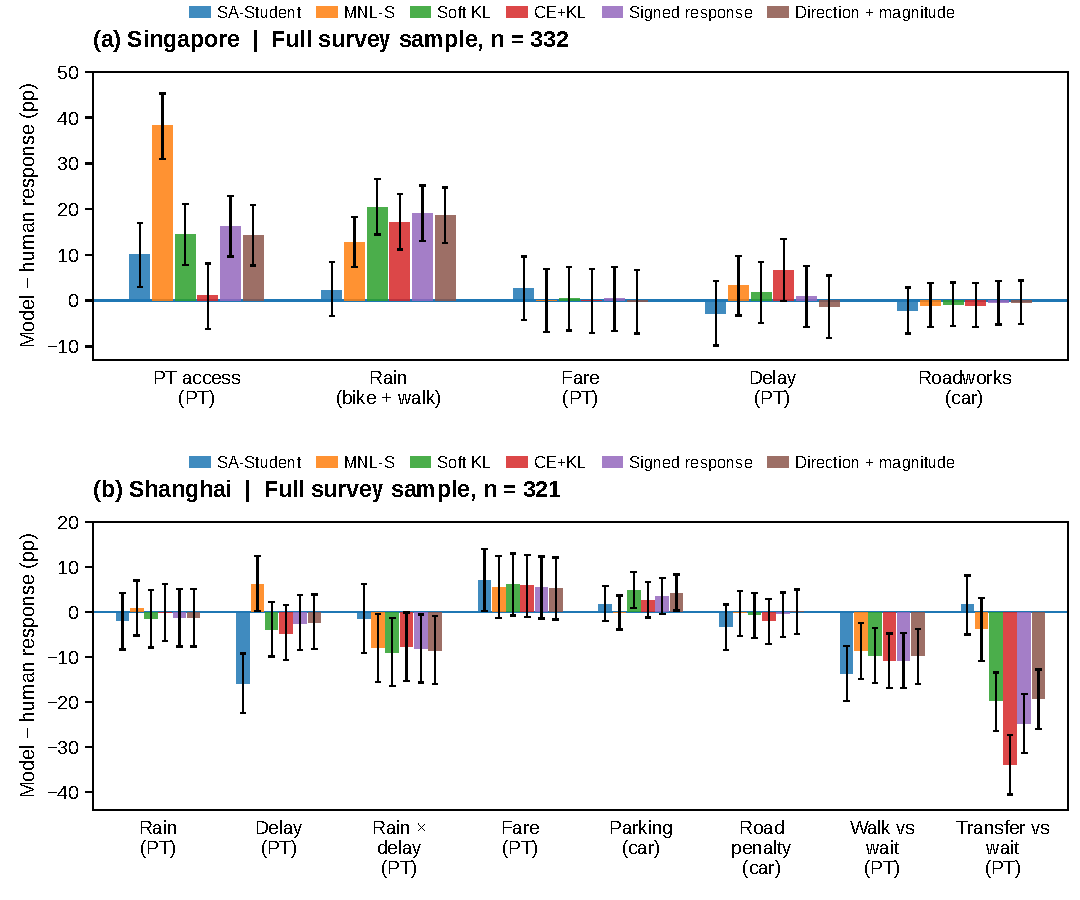
\includegraphics[width=0.94\textwidth]{figures/narrative/figure4_human_response.pdf}
\caption{Response differences in the full samples, defined as the change in model probability minus the change in stated-choice share. Whiskers show Bonferroni-adjusted respondent-bootstrap intervals within each city (99\% for Singapore and 99.375\% for Shanghai). Neural means average three fitted seeds. Shanghai results use the reference specification of Section~\ref{sec:human_design}. The interaction and walking-versus-waiting contrasts include 320 respondents.}
\label{fig:human_response}
\par\vspace{9pt}
\begin{resulttable}
\caption{Choice accuracy, PT share bias and mean absolute response bias against stated choices.}
\label{tab:human_main}
\setlength{\tabcolsep}{3pt}
\renewcommand{\arraystretch}{1.12}
\begin{tabular*}{\linewidth}{@{\extracolsep{\fill}}lrrrrrr@{}}
\toprule
& \multicolumn{3}{c}{Singapore ($n=332$)} & \multicolumn{3}{c}{Shanghai ($n=321$)} \\
\cmidrule(lr){2-4}\cmidrule(l){5-7}
Model & Acc. (\%) & PT bias (pp) & Mean $|B_c|$ & Acc. (\%) & PT bias (pp) & Mean $|B_c|$ \\
\midrule
SA-Student & $66.9$ & $-30.7$ & $4.0$ & $80.5$ & $-16.8$ & $5.8$ \\
MNL-S & $71.1$ & $-3.8$ & $11.1$ & $81.8$ & $-5.4$ & $4.1$ \\
Soft KL & $72.9\,\pm\,0.9$ & $-17.7\,\pm\,3.3$ & $8.2\,\pm\,3.3$ & $78.5\,\pm\,1.7$ & $-12.3\,\pm\,7.9$ & $7.6\,\pm\,0.9$ \\
CE+KL & $69.7\,\pm\,0.3$ & $-23.5\,\pm\,3.5$ & $6.9\,\pm\,1.7$ & $77.1\,\pm\,3.0$ & $-15.0\,\pm\,6.8$ & $9.1\,\pm\,1.9$ \\
Signed response & $73.1\,\pm\,1.2$ & $-16.0\,\pm\,3.5$ & $8.6\,\pm\,3.0$ & $79.8\,\pm\,1.1$ & $-10.7\,\pm\,6.2$ & $7.7\,\pm\,1.8$ \\
Direction+magnitude & $71.8\,\pm\,3.1$ & $-16.7\,\pm\,6.2$ & $8.8\,\pm\,2.0$ & $80.3\,\pm\,0.5$ & $-10.4\,\pm\,5.9$ & $7.5\,\pm\,1.0$ \\
\bottomrule
\end{tabular*}
\par\smallskip\begin{minipage}{\linewidth}\footnotesize
All 3,320 Singapore and 3,208 Shanghai explicit choices are scored, including eight and two choices of modes the model treats as unavailable. PT bias is the mean predicted PT probability minus the stated PT share. Mean $|B_c|$ is computed within each fitted seed by taking the absolute bias for each contrast and averaging over the five Singapore or eight Shanghai contrasts; these seed-level metrics are then averaged. Figure~\ref{fig:human_response} instead plots signed biases averaged over seeds, whose absolute values need not equal the table metric. Both are in percentage points. Neural entries are means $\pm$ SD over three training seeds. Always predicting PT gives accuracies of 66.57\% and 71.98\%. Further metrics are given in Supplementary Table~\ref{supp-tab:human_primary}.
\end{minipage}
\end{resulttable}

\end{figure}
How well a Student agrees with people depends on the intervention. In Singapore, SA-Student predicts a PT-delay response of $-14.86$ percentage points, compared with a stated change of $-12.05$ points, a bias of $-2.81$ points (nominal 95\% interval $[-8.18,2.75]$). Rain lowers its bicycle-plus-walk probability by 19.70 points, close to the 21.99-point fall in stated choice. Poorer PT accessibility is a different case. The Student predicts a change of $-14.42$ points against a stated $-24.40$, and the resulting $+9.98$-point bias remains positive after adjustment for multiple contrasts ($[3.01,16.93]$).

Shanghai reverses the pattern for delay. Under the reference specification, SA-Student predicts a PT-delay response of $-30.57$ points, roughly twice the stated $-14.64$. The bias of $-15.93$ points excludes zero after adjustment over eight contrasts ($[-22.41,-9.21]$). The Student also predicts responses of the wrong sign for the fare and walking-versus-waiting contrasts (Figure~\ref{fig:human_response}). These discrepancies persist across the eight alternative input specifications, where the delay bias ranges from $-16.53$ to $-10.25$ points and both sign reversals remain. These specifications retain the 15-minute encoding of the qualitative delay condition; they do not test sensitivity to its intensity.

The ranking of objectives on the Teacher benchmark does not carry over to people. In Singapore, direction+magnitude shifts the delay bias from $+1.78$ points under soft KL to $-1.34$, yet both objectives substantially understate the rain response. MNL-S offers the clearest example. It approximates the Singapore fare response and the Shanghai parking and road responses, but under poorer Singapore accessibility it predicts a PT change of $+13.85$ points, whereas the stated PT share falls by 24.40 points. The accessibility task raises PT travel time from 32 to 48 minutes, access walking from three to twelve minutes and transfers from zero to two (Supplementary Table~\ref{supp-tab:survey_tasks}). The reversal thus concerns this combined access burden rather than any single walking-time coefficient. The model with the smallest Teacher error is, for this intervention, the only one that predicts the wrong direction. Conversely, CE+KL, which has the largest Teacher-response error, comes closest to the stated accessibility response ($-23.37$ against $-24.40$ points; Supplementary Table~\ref{supp-tab:responses_singapore_0}).

Response bias and level bias also rank the models differently (Table~\ref{tab:human_main}). SA-Student underpredicts the PT share by 30.67 points in Singapore and 16.84 in Shanghai, whereas MNL-S narrows these gaps to 3.77 and 5.36 points. In Singapore, however, MNL-S has the larger mean absolute response bias, 11.1 points against 4.0 for SA-Student. A model can therefore reproduce how many people use PT while misrepresenting how that number changes, and the reverse also occurs. Accuracy is a weak guide in either case. SA-Student's accuracy of 66.93\% in Singapore barely exceeds the 66.57\% obtained by always predicting PT, while in Shanghai it reaches 80.46\%.

Numerical inputs affect agreement as well, though not mainly through respondent-specific matching. In Shanghai, replacing reference values with network-derived inputs raises accuracy by 2.80 percentage points, and the gain remains 2.56 points after assigning fresh origin--destination pairs and 2.52 points after exchanging complete supply profiles between respondents. Most of the improvement therefore comes from a general shift in the numerical inputs rather than from matching them to individual respondents (Supplementary Section~\ref{supp-sec:od_sensitivity}).

\subsection{Discrepancies relative to a contemporary API reference}
\label{sec:teacher_results}
The matched 24-person subsets describe two components of discrepancy under the reference inputs (Figure~\ref{fig:teacher_attribution}). They compare current predictions and do not identify the historical origin of the differences. The first component is the contemporary Teacher--human discrepancy. Under poorer accessibility, the selected Singapore respondents reduce PT choice by 37.50 points, while the contemporary Teacher predicts a reduction of 15.40 points and SA-Student 13.46. The attenuation is also observed in the contemporary Teacher, and SA-Student differs from it by $+1.94$ points (nominal 95\% interval $[-3.40,7.26]$).

The second component is the Student--Teacher discrepancy. For the encoded Shanghai delay task, the selected respondents and the Teacher agree closely, at $-8.33$ and $-8.17$ points, but SA-Student predicts $-34.87$. Its difference from the Teacher is $-26.70$ points, with a family-adjusted interval of $[-36.95,-15.42]$. The other Students respond less strongly, at $-19.03$ for soft KL, $-17.17$ for direction+magnitude and $-8.85$ for MNL-S, so SA-Student shows the largest discrepancy in this comparison. This pattern does not isolate its training history from changes in the Teacher service.

\begin{figure}[pos=H]
\centering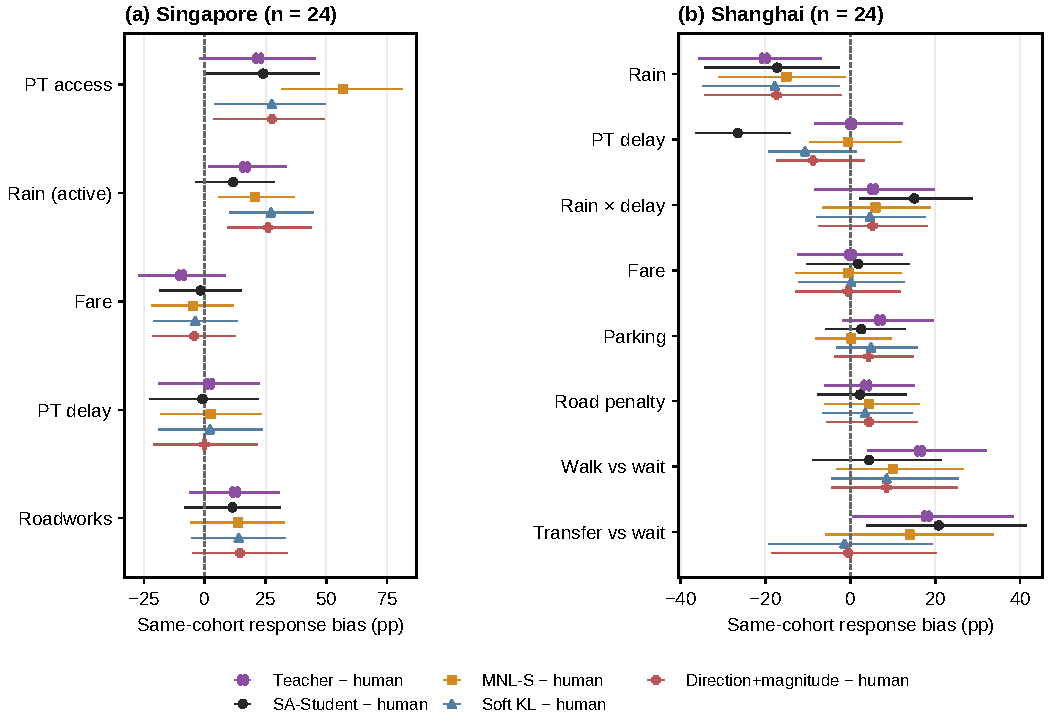
\includegraphics[width=0.88\textwidth]{figures/narrative/figure5_teacher_comparison.pdf}
\caption{Contemporary API reference and Student response differences on the matched 24-person subsets. The Teacher label denotes the current API reference, not a verified reconstruction of the training backend. Points show the change in model probability minus the change in stated-choice share, and bars show nominal 95\% respondent-bootstrap intervals. Teacher means average three elicitations per state, and controlled neural means average three fitted seeds. Paired intervals between Student and Teacher are given in Table~\ref{tab:teacher_decomposition_s9} and the supplement.}
\label{fig:teacher_attribution}
\end{figure}

The two terms of Eq.~\ref{eq:attribution} can also offset each other (Table~\ref{tab:teacher_decomposition_s9}). In the Shanghai walking-versus-waiting contrast, the Teacher exceeds the human response by $+16.31$ points and SA-Student falls $11.88$ points below the Teacher, leaving a total bias of only $+4.43$ points. A small total bias can therefore conceal two larger, opposing discrepancies. For this reason the decomposition is more informative than the total bias for distinguishing the two observed discrepancies, although the Student--Teacher term may also include changes in the Teacher since training.

\begin{table}[pos=H]
\centering\small
\caption{Decomposition of signed response differences among stated choices, the contemporary Teacher and SA-Student.}
\label{tab:teacher_decomposition_s9}
\setlength{\tabcolsep}{3pt}
\renewcommand{\arraystretch}{1.12}
\begin{tabular*}{\linewidth}{@{\extracolsep{\fill}}lrrr@{}}
\toprule
Contrast & Teacher $-$ human & SA-Student $-$ Teacher & SA-Student $-$ human \\
\midrule
\multicolumn{4}{l}{\textit{Singapore ($n=24$)}} \\
Poorer PT access & $+22.1\;[-9.9, 52.1]$ & $+1.9\;[-4.9, 9.1]$ & $+24.0\;[-7.2, 54.3]$ \\
Rain (active modes) & $+16.7\;[-2.4, 38.4]$ & $-5.0\;[-11.4, 1.1]$ & $+11.7\;[-8.0, 33.9]$ \\
PT fare & $-9.6\;[-33.4, 14.8]$ & $+7.8\;[4.1, 12.4]$ & $-1.8\;[-26.2, 22.6]$ \\
PT delay & $+1.9\;[-25.2, 28.9]$ & $-2.9\;[-12.3, 5.8]$ & $-0.9\;[-28.8, 29.7]$ \\
Road penalty & $+12.5\;[-12.0, 36.3]$ & $-1.0\;[-5.8, 4.2]$ & $+11.4\;[-14.8, 37.0]$ \\
\midrule
\multicolumn{4}{l}{\textit{Shanghai ($n=24$)}} \\
Rain & $-20.2\;[-41.6, -2.5]$ & $+3.0\;[-2.9, 8.0]$ & $-17.2\;[-41.5, 2.3]$ \\
PT delay & $+0.2\;[-10.2, 18.0]$ & $-26.7\;[-36.9, -15.4]$ & $-26.5\;[-39.3, -8.3]$ \\
Rain $\times$ delay & $+5.3\;[-13.9, 26.1]$ & $+9.7\;[3.3, 16.2]$ & $+15.0\;[-2.5, 34.7]$ \\
PT fare & $+0.0\;[-16.8, 16.7]$ & $+1.8\;[0.3, 3.2]$ & $+1.8\;[-14.6, 18.3]$ \\
Parking & $+7.0\;[-3.0, 24.6]$ & $-4.5\;[-11.0, -0.3]$ & $+2.6\;[-8.1, 17.7]$ \\
Road penalty & $+3.8\;[-10.3, 20.1]$ & $-1.5\;[-4.7, 0.7]$ & $+2.2\;[-11.6, 18.3]$ \\
Walk versus wait & $+16.3\;[0.2, 39.6]$ & $-11.9\;[-14.2, -9.1]$ & $+4.4\;[-13.0, 29.2]$ \\
Transfer versus wait & $+17.9\;[-7.4, 44.4]$ & $+2.9\;[0.4, 5.2]$ & $+20.8\;[-4.0, 46.8]$ \\
\bottomrule
\end{tabular*}
\par\smallskip\begin{minipage}{\linewidth}\footnotesize
Entries are percentage points with Bonferroni-adjusted respondent-bootstrap intervals, computed within each city over five Singapore or eight Shanghai contrasts. All terms use the same respondents, the same fitted SA-Student and Teacher means over three elicitations. Point estimates are rounded to one decimal place. The SA-Student $-$ Teacher term may include changes in the Teacher since training.
\end{minipage}
\end{table}


\FloatBarrier
\subsection{Response transmission through assignment and execution}
\label{sec:execution_results}
For SA-Student in Helsinki, the predicted response to perceived PT delay is $-13.10$ percentage points. Deterministic assignment gives $-13.00$ points, and routed modes and simulated PT use both give $-12.30$. The resulting gap of $+0.80$ points has a paired-person 95\% interval of $[-0.77,2.38]$. The level of PT use behaves very differently. At baseline, mean PT probability is 27.74\%, 218 of the 1,000 travelers are assigned PT, and 161 board PT in the simulation, so 73.85\% of assigned PT users board before reaching the outbound destination. PT use thus falls by more than eleven points between prediction and simulation, while the delay response changes by less than one point. The distinction between levels and responses that separates static from response fidelity thus reappears at the network stage.
\begin{figure}[pos=!ht]
\centering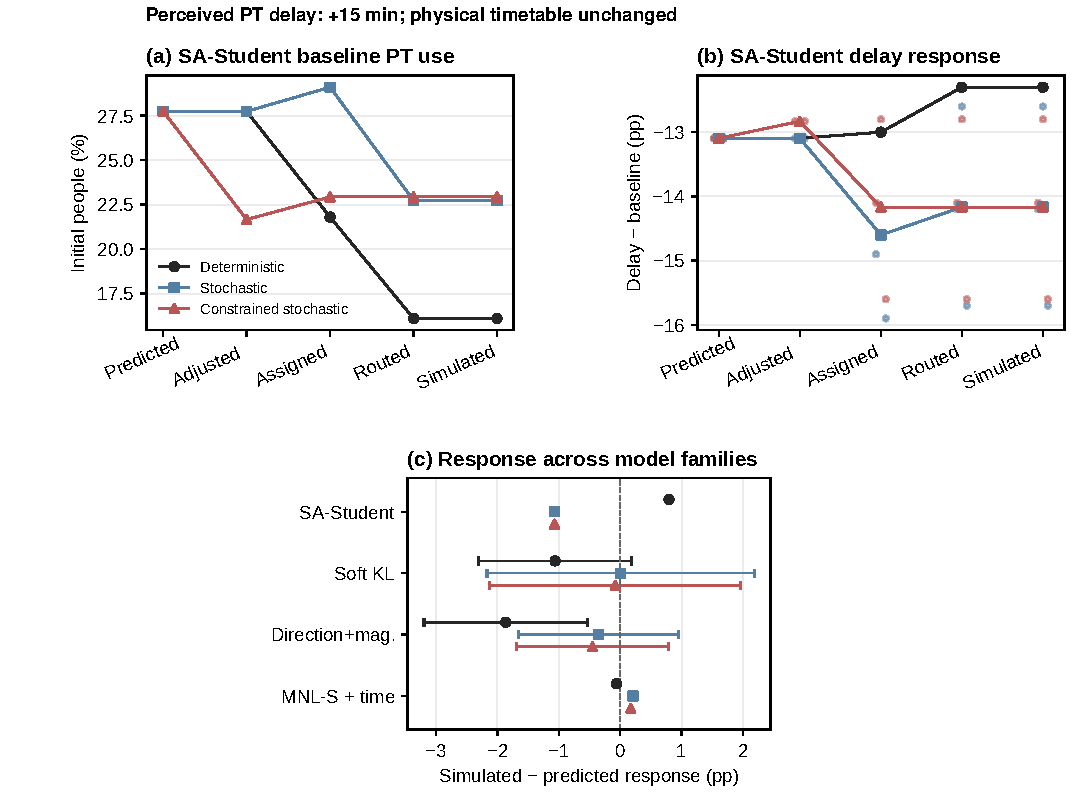
\includegraphics[width=0.87\textwidth]{figures/narrative/figure6_execution_response.pdf}
\caption{Response preservation for a fixed population of 1,000 Helsinki travelers under a 15-minute perceived PT delay, with the physical timetable unchanged. (a,b) Baseline PT shares and delay responses of SA-Student across predicted probabilities, feasibility-adjusted probabilities (Adjusted), assigned modes, routed modes and simulated PT use. Small points in (b) show individual assignment seeds. (c) Predicted-to-simulated gaps by model family. Error bars show training-seed SD after averaging assignment repetitions within each model. Simulated PT use is defined by boarding and does not require journey completion.}
\label{fig:execution_response}
\end{figure}

Stochastic assignment represents the predicted distribution in expectation, but a finite population still varies from draw to draw. For SA-Student, ordinary and feasibility-constrained sampling both give a mean simulated response of $-14.17$ points, with assignment SDs of 1.55 and 1.40 points. Feasibility adjustment changes the probability response to $-12.83$ points and prevents PT assignments for which the specified search finds no route. It makes the assigned demand routable, but it does not bring the simulated response closer to the original prediction in this population. Routability and response preservation are separate properties of an assignment rule. Eq.~\ref{eq:execution_decomposition} further separates their contributions: for the feasibility-constrained SA-Student result, the reported mean responses imply a $+0.27$-point shift from prediction to adjusted probabilities and a $-1.34$-point shift from adjusted probabilities to simulation, summing to the $-1.07$-point total gap. These differences are calculated from the reported rounded means; their component uncertainties are not estimated separately here.
\begin{table}[pos=!ht]
\centering\small
\caption{Predicted and simulated PT responses in the fixed 1,000-person Helsinki population.}
\label{tab:execution_main}
\setlength{\tabcolsep}{3pt}
\renewcommand{\arraystretch}{1.12}
\begin{tabular*}{\linewidth}{@{\extracolsep{\fill}}llrrrr@{}}
\toprule
Model & Assignment & Predicted (pp) & Simulated (pp) & Gap (pp) & Assignment SD \\
\midrule
SA-Student & Deterministic & $-13.10$ & $-12.30$ & $0.80$ & -- \\
SA-Student & Stochastic & $-13.10$ & $-14.17$ & $-1.07$ & 1.55 \\
SA-Student & Constrained & $-13.10$ & $-14.17$ & $-1.07$ & 1.40 \\
Soft KL & Deterministic & $-6.97\pm4.92$ & $-8.03\pm5.13$ & $-1.06\pm1.24$ & -- \\
Soft KL & Stochastic & $-6.97\pm4.92$ & $-6.97\pm3.32$ & $0.01\pm2.18$ & 0.27 \\
Soft KL & Constrained & $-6.97\pm4.92$ & $-7.06\pm3.41$ & $-0.08\pm2.04$ & 0.28 \\
Direction+magnitude & Deterministic & $-6.77\pm4.96$ & $-8.63\pm4.76$ & $-1.87\pm1.33$ & -- \\
Direction+magnitude & Stochastic & $-6.77\pm4.96$ & $-7.12\pm3.97$ & $-0.35\pm1.30$ & 0.35 \\
Direction+magnitude & Constrained & $-6.77\pm4.96$ & $-7.22\pm4.06$ & $-0.45\pm1.24$ & 0.32 \\
MNL-S + neural time & Deterministic & $-6.84\pm0.00$ & $-6.90\pm0.00$ & $-0.06\pm0.00$ & -- \\
MNL-S + neural time & Stochastic & $-6.84\pm0.00$ & $-6.63\pm0.00$ & $0.21\pm0.00$ & 1.10 \\
MNL-S + neural time & Constrained & $-6.84\pm0.00$ & $-6.67\pm0.00$ & $0.17\pm0.00$ & 1.21 \\
\bottomrule
\end{tabular*}
\par\smallskip{\footnotesize Responses are changes in PT use from baseline to perceived delay over the same 1,000 people, with the physical timetable unchanged. Gap is the simulated minus the predicted response. Constrained denotes feasibility-constrained stochastic assignment. Values average assignment repetitions within each fitted model and then across models, and $\pm$ gives the SD across three training seeds. SA-Student is a single fitted model. Assignment SD is the mean within-model SD across assignment repetitions. Intermediate stages and absolute-gap summaries are given in Supplementary Tables~\ref{supp-tab:execution_layers}--\ref{supp-tab:execution_gap_aggregation}.}
\end{table}


MNL-S with neural timing predicts $-6.84$ points and yields $-6.90$ under deterministic assignment (Table~\ref{tab:execution_main}). Its stochastic and feasibility-constrained means are $-6.63$ and $-6.67$. For a given assignment seed, PT use is identical across its three independently fitted timing predictors, so timing variability does not alter this model's simulated mode response.

Signed averages can hide opposing errors. The stochastic-assignment gap of soft KL averages approximately zero across fitted models, but the model-specific means range from $-2.17$ to $+2.18$ points. When assignment repetitions are averaged within each fitted model before taking absolute values, the mean absolute gap is 1.45 points for soft KL and 0.91 for direction+magnitude (Supplementary Table~\ref{supp-tab:execution_gap_aggregation}). In this summary, the objective that preserves Teacher responses better also reaches the network with smaller model-specific gaps, a difference that the signed mean conceals.

Departure timing affects routing even when feasibility does not change. Applying SA-Student's predicted departure adjustment alters the selected itinerary in 279 baseline and 313 delay cases while leaving binary PT feasibility unchanged. The timing output therefore shapes the schedule that travelers meet in the simulation, an effect that a feasibility check alone would not reveal.

Journey times depend on the representation of the network as well as on mode counts. In the Shanghai speed experiment, PT counts stay at 224 at baseline and 134 under delay, and all 321 people complete their journeys. The paired change in outbound time is nevertheless $-4.44$ minutes with network-derived active-mode speeds and $+14.04$ minutes with mode-specific speed caps for walking and cycling, the latter with an interval of $[11.18,17.05]$ minutes. Identical demand plans can thus imply time changes of opposite sign (Supplementary Section~\ref{supp-sec:speed_sensitivity}).

\FloatBarrier
\subsection{Computational implications for scenario analysis}
In the measured post-training builds, local behavioral prediction accounts for less than one percent of scenario-construction time. Constructing a scenario for 10,000 Singapore agents takes 51.1 minutes, of which behavioral prediction accounts for 10.3 seconds. For 50,000 agents the corresponding times are 231.8 minutes and 48.8 seconds, so inference contributes approximately 0.34\% and 0.35\% of construction time. In a model-only benchmark that excludes feature encoding and routing, MNL-S with neural timing requires $1.68\pm0.33$ microseconds per state, compared with 1.78--2.16 microseconds for the joint neural objectives.

The dominant cost lies in network and timetable calculations. Reusing those that do not change between scenarios reduces construction time from 3,223.6 to 469.5 seconds in Singapore and from 10,491.8 to 103.2 seconds in Helsinki, with mode and origin--destination assignments unchanged. Each city was measured under one reuse condition, and concurrent workload limits the precision of these timings. The differences among compact Students are negligible by comparison.

The archived usage records also permit a monetary estimate without new Teacher calls (Table~\ref{tab:api_cost}). Across the retained archives, 13,391 deduplicated completions with usage consumed 17.157 million input and 50.418 million output tokens. Repricing them at the official V4 Pro rates gives US\$102.71--205.42; the final same-task reference accounts for US\$7.08--14.16. These are rate-card scenarios for observed usage, not provider invoices or a complete lifecycle total. In particular, 576 earlier completions lack usage, and the retained archives do not cover every failed attempt or acquisition source. Reasoning tokens are already included in output tokens.
\begin{table}[pos=htbp]
\centering\small
\caption{Retained API usage repriced at the official DeepSeek V4 Pro rates checked on 25 September 2026. Costs are estimates in USD, not invoices.}
\label{tab:api_cost}
\setlength{\tabcolsep}{3pt}
\begin{tabularx}{\linewidth}{@{}Xrrrr@{}}
\toprule
Acquisition group & Metered calls & Input (M) & Output (M) & USD range \\
\midrule
Primary supervision archives & 8,681 & 10.050 & 32.614 & 65.83--131.66 \\
Final same-task reference & 1,440 & 2.324 & 3.255 & 7.08--14.16 \\
Earlier same-task campaign & 1,475 & 1.969 & 5.575 & 11.58--23.15 \\
Neutral-metadata pilot & 120 & 0.160 & 0.239 & 0.52--1.03 \\
Ownership pilot & 120 & 0.160 & 0.235 & 0.52--1.03 \\
Latency benchmark & 87 & 0.117 & 0.353 & 0.76--1.51 \\
Other historical development & 1,468 & 2.377 & 8.149 & 16.43--32.86 \\
Retained metered total & 13,391 & 17.157 & 50.418 & 102.71--205.42 \\
\bottomrule
\end{tabularx}
\par\smallskip\begin{minipage}{\linewidth}\footnotesize
Completion IDs are deduplicated across archives. Input costs use the recorded cache-hit/miss split; output includes reasoning tokens. The range reprices the same usage entirely at off-peak or peak rates, rather than reconstructing historical deductions. The primary archives contain the legacy, joint and corrected accessibility acquisition pools, including labels outside the final benchmark. Other development includes deprecated S8. A further 576 retained completions lack usage and are excluded from the monetary sum, as are unmetered failures; their cost is unknown. The earlier same-task campaign includes 35 responses rejected by parsing but with recorded token usage. This is neither the marginal cost of one fitted Student nor a full project invoice.
\end{minipage}
\end{table}


For repeated deployment, let $C_0$ denote acquisition, retry, training and necessary adaptation costs, and let $c_L$ and $c_S$ be the monetary costs of evaluating the same scenario directly with the LLM and with the Student. The break-even workload is
\begin{equation}
 N^*=\frac{C_0}{c_L-c_S},\qquad c_L>c_S.
 \label{eq:break_even}
\end{equation}
Shared feature, supply and routing work must be counted consistently in both pipelines, with matching caching and concurrency assumptions. Existing inference, construction and token records support the components above, but the missing acquisition charges and local-compute tariff prevent a measured lifecycle break-even claim. Wall-clock and resource break-even require separate calculations in their own units; successful-request latency cannot replace elapsed campaign time (Supplementary Section~\ref{supp-sec:supp_compute}).
\FloatBarrier

\section{Discussion}
\label{sec:discussion}
\subsection{Response fidelity is a separate model-selection criterion}
The central result is not that a particular loss or architecture wins every comparison. It is that Teacher-response fidelity, agreement with stated choices and execution consistency rank models differently. In the controlled benchmark, explicit response weighting improves finite-contrast error, but changing the choice specification produces a larger gain. The signed and direction+magnitude objectives are not clearly separated by the paired interval, and neither improves interaction error over soft KL. The evidence therefore supports evaluating and weighting responses, without establishing that the split sign--magnitude construction is essential.

This interpretation follows the information structure of the experiment. The same endpoint targets are available to every controlled model, and Eq.~\ref{eq:bound} connects their errors to response error. Paired supervision reallocates optimization effort across those errors rather than revealing additional Teacher behavior. Results across the six held-out personas and the available Teacher reaggregations support the within-benchmark comparison. Transfer to unseen intervention families, intensities or Teachers remains a separate empirical question.

MNL-S's advantage makes model specification an important control rather than a secondary baseline. Its linear utilities provide inspectable coefficients, and separate neural timing retains most of the timing accuracy of joint models. This combination supports modular estimation and later recalibration. It does not establish that travelers follow linear utilities or that every coefficient has an economically valid interpretation: the choice target is an LLM judgment, and smoothness or regularization could also explain the gain. Behavioral interpretation requires checking identified utility differences, relevant signs and implied sensitivities, not merely naming the model logit.

\subsection{Human agreement requires an independent empirical test}
Teacher fidelity is not a proxy for agreement with people. MNL-S reverses the stated Singapore accessibility response, whereas CE+KL, the least faithful controlled objective, comes closest to that contrast. Baseline levels and responses also separate: SA-Student understates Singapore PT use by about 31 percentage points yet has the smallest mean absolute response bias there; MNL-S comes within four points of the PT share but misses important changes. These observations extend the distinction between predictive and behavioral criteria \citep{wang2020deep,martinbaos2023prediction} to models compressed from LLM judgments.

The contemporary API reference helps identify where follow-up tests are needed, without assigning historical causation. For Singapore accessibility, it also attenuates the stated response, so bringing SA-Student closer to that reference would leave substantial human disagreement. For Shanghai delay under the reference encoding, the current model is close to the human point estimate while SA-Student responds much more strongly. The second pattern motivates a controlled check of Student specification and input encoding; it does not establish that compression caused the discrepancy. The Shanghai walking-versus-waiting result additionally illustrates cancellation: a small total bias can combine larger opposing Student--reference and reference--human terms.

This distinction suggests two different development tasks. Compression should be evaluated against frozen Teacher targets. Empirical alignment should be fitted and selected using separate human data, then tested on people and tasks not used for that alignment, as motivated by recent travel-choice and travel-satisfaction research \citep{liu2026persona,xu2026satisfaction}. The surveys in the present study were reserved for evaluation, so the observed differences diagnose calibration needs rather than demonstrate a calibrated traveler model.

\subsection{Routability, response transmission and practical use}
The Helsinki experiment isolates what happens after behavioral prediction. For SA-Student, baseline PT use falls by more than eleven points between prediction and boarding while the deterministic delay response changes by less than one point. A small response gap can thus coexist with a substantial level gap. Feasibility-constrained assignment removes PT choices for which the specified search finds no connection, yet does not reduce the response gap for this population. Routability and preservation of a prescribed behavioral distribution are different objectives.

The stagewise accounting makes these differences auditable. All shares use the same initial population; predicted and adjusted probabilities remain distinct from assigned modes, routed modes and boarding events. Signed and absolute gaps are both needed because cancellation across fitted models can conceal errors. Timing outputs also warrant separate evaluation: they change itineraries even when binary feasibility remains unchanged. The additional speed experiment shows why a stable mode count alone cannot validate a journey-time outcome.

For implementation, the relevant efficiency result concerns repeated use after training. Behavioral inference consumes approximately 0.35\% of the measured larger scenario builds, shifting attention to supply calculation and reuse rather than marginal differences between compact Students. The retained token ledger quantifies an additional acquisition-cost component, but it does not yet determine the lifecycle break-even workload: unmetered attempts and local-compute costs remain outside the estimate in Table~\ref{tab:api_cost}.

\subsection{Scope of inference and next tests}
Three boundaries define the conclusions. First, the compression comparison uses one archived Teacher and six held-out synthetic personas. Teacher reaggregation and seed variation test sensitivity within that design; they do not substitute for new personas, unseen interventions or another frozen Teacher. Second, the human evidence concerns stated responses in two convenience samples under documented encodings. The cities used different task formats, Shanghai's qualitative tasks require numerical reference values, and the existing sensitivity analysis holds its delay at 15 minutes. Explicit currency, alternative-set interpretation and randomized, numerically matched tasks are priorities for further validation. Third, Helsinki holds physical supply and behavioral predictions fixed to isolate execution effects. Physical service changes and feedback from experienced conditions require separate experiments before extending the conclusions to equilibrium or operational disruption forecasting.

These boundaries define a usable validation sequence rather than a single pass/fail imitation score: specify the intervention and output; test compression against archived targets; compare the corresponding human response; and audit the outcome after assignment and execution. A failure at one level identifies the next model component or evidence source to examine. Supplementary Section~\ref{supp-sec:materials_scope} provides the versioned material inventory and distinguishes reproducible target-based evaluation from live-API and restricted-data dependencies.

\section{Conclusion}
\label{sec:conclusion}
This study evaluates LLM-derived traveler models through finite responses rather than baseline imitation alone. On the controlled benchmark, response-aware supervision improves Teacher fidelity and a logit choice model with independent neural timing performs better still on response error. That ranking does not carry over to the stated-choice samples: the Teacher-best Student reverses a human accessibility response. In the controlled Helsinki execution experiment, improved routability likewise does not ensure closer transmission of the predicted response.

The practical contribution is a response-centric validation procedure linking compression, empirical comparison and network execution. Each level answers a different question, and success at one cannot stand in for evidence at another. A traveler model intended for a specified intervention should therefore be evaluated on its response at all relevant levels, with baseline demand and computational cost reported separately. The current evidence establishes these distinctions within the tested Teacher, samples and execution setting; broader forecasting claims require the corresponding out-of-setting tests.

\section*{Data and code availability}
Code, prepared synthetic benchmark states and targets, split manifests, selected Student checkpoints, evaluation scripts and compact result tables are included in the research repository, \url{https://github.com/AnXu-ITS/DeepSeek_Traveler_Behavior_Distillation_Research}. The experimental artifacts are pinned to the 24 September 2026 repository edition at commit \texttt{4e67286}; the 25 September editorial revision adds aggregate cost accounting and corrected service and consent statements without new experiments. The complete base identifier and material inventory are given in Supplementary Section~\ref{supp-sec:materials_scope}. Archived targets permit controlled-model evaluation without new Teacher calls. The repository remains access-controlled; requests should be directed to the corresponding author. Participant-level survey records and participant-linked API payloads are retained separately, subject to privacy and applicable permissions. The repository includes Helsinki run-level summaries and analysis code; fresh simulation additionally requires the documented supply files and MATSim environment. Supplementary Section~\ref{supp-sec:materials_scope} specifies the coverage of each reproduction task.
\bibliographystyle{cas-model2-names}
\bibliography{references}
\end{document}
